\documentclass{beamer}

\usetheme{default}
\usecolortheme{default}
\usefonttheme{default}
\setbeamertemplate{navigation symbols}{} % Remove navigation symbols

\title{Role of AI in Next Generation\\ Impact Based Forecasting for Floods}
\author{Dr. Nishadh Kalladath}
\institute{DRM Program\\ IGAD Climate Prediction and Applications Centre - ICPAC}
\date{October 22, 2023}
%\logo{%
%	\includegraphics[width=1cm,height=1cm,keepaspectratio]{icpac-logo.png}\hspace*{0.1cm}%
%	\includegraphics[width=1cm,height=1cm,keepaspectratio]{norcap-logo.png}%
%}

\titlegraphic{
	\includegraphics[width=1cm]{icpac-logo.png}
	\hspace*{0.1cm}%
	\includegraphics[width=1cm]{norcap-logo.png}
}



\usepackage{tikz}
\usepackage[absolute,overlay]{textpos}
\setbeamertemplate{navigation symbols}{} % optional: suppresses navigation symbols

\usepackage{caption}
\captionsetup[figure]{name={}}


\usepackage{color}

\usetikzlibrary{positioning}

\begin{document}

\begin{frame}
    \maketitle
    %\frametitle{Title}
%    \hfill
%    \includegraphics[width=0.09\textwidth]{icpac-logo.png} % Assuming you have the logo named as 'IGADlogo.png'
%    \includegraphics[width=0.1\textwidth]{norcap-logo.png} % Assuming you have the logo named as 'NORCAPlogo.png'

\footnotesize{* Presented at TH01: Artificial Intelligence for climate risk mitigation: navigating opportunities and challenges, 22 October 2023, WCP OSC-2023}
\end{frame}

%Background to IBF and what are its next generations​
%
%Why next generation​
%
%Reason1- Tim​
%
%Reason2- Nassim​
%
%Reason3- BN book​
%
%Role of AI for IBF​
%
%Summmary of change needed​
%
%Post processing of ens forecat​
%
%Random egenrator parsimomnous model​
%
%Baysian Netowkr ​
%
%Storylines ​
%
%Key takeaways ​
\begin{frame}{Table of Contents}
	\tableofcontents
\end{frame}

\section{Generations of IBF}	

\begin{frame}
	\frametitle{Impact Based Forecasting}
	\begin{figure}[h]
		\centering
	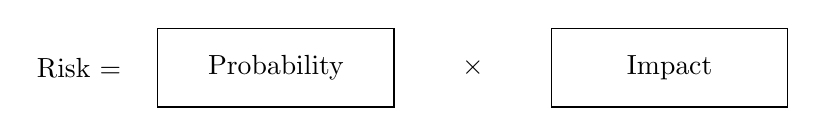
\begin{tikzpicture}
		
		% Draw the boxes
		\node[draw, minimum width=3cm, minimum height=1cm, align=center] at (0,0) {Probability};
		\node[draw, minimum width=3cm, minimum height=1cm, align=center] at (5,0) {Impact};
		
		% Place the equation components
		\node at (-2.5,0) {Risk =};
		\node at (2.5,0) {$\times$};
		
	\end{tikzpicture}
\caption{Standard Impact Based Risk Measure}
\label{fig:my_tikz}
\end{figure}


\begin{figure}
	\includegraphics[width=1.0\linewidth]{risk-mat.png} 
	\caption{Impact communication through risk matrices}
\end{figure}
\end{frame}

\begin{frame}
	\frametitle{Impact Based Forecasting}
	\begin{figure}
		\includegraphics[width=1.0\linewidth]{ibf-type.png} 
		\caption{Typical workflow of IBF}
	\end{figure}
\vspace{1em}

\textcolor{blue}{\textbf{Characteristics of IBF}}
%\section{Characteristics of IBF}
\begin{itemize}
	\item Impact Based Risk Measure
	\item As a risk communication tool
	\item Risk and Decision Analysis tool
	\item Reasoning under uncertainty
\end{itemize}

\end{frame}


\begin{frame}
	\frametitle{Different Generations of IBF*}
	\begin{enumerate}
		\item Deterministic Forecasts - Current Generation
		\item Probabilistic Forecasts - Conditional probability 
		\item Storylines - Deep uncertainty
   \end{enumerate}	

\textcolor{blue}{\textbf{Limitations of Current Generation}}
%\section{Characteristics of IBF}
\begin{itemize}
	\item Not based on Ensemble forecasts
	\item Overlook conditional elements, 
	\item Not evaluate potential interventions and consequences of varied actions
\end{itemize}

		
	 \vspace{10em}
	\footnotesize{* Simpson, Michael, et al. "Decision analysis for management of natural hazards." Annual Review of Environment and Resources 41 (2016): 489-516.}
	
	
	
\end{frame}

\section{Why Next Generations}

\begin{frame}
\frametitle{Why Next Generations: The Primacy of Doubt}

\begin{columns}
	
	% Left column
	\begin{column}{0.75\textwidth}
		\begin{itemize}
			\item Limitations of deterministic forecast 
			\item Need of Ensemble forecast
			\item Theory behind storyline method 
		\end{itemize}
	\end{column}
	
	% Right column
	\begin{column}{0.5\textwidth}
		\includegraphics[width=0.6\linewidth]{primacy.png} \\
		\tiny{Tim Palmer on Doubt: From Quantum Physics to Climate Change | Closer To Truth Chats}
		\vspace{1cm}
		\includegraphics[width=0.8\linewidth]{tim1.png} \\
	\end{column}
	
\end{columns}

\end{frame}

\begin{frame}
	\frametitle{How to use ensemble forecast}
%	\begin{figure}
%		\includegraphics[width=1.0\linewidth]{ensemble_weather_forecast.png} 
%		%\caption{Typical output of IBF}
%	\end{figure}

\begin{tikzpicture}[remember picture,overlay]
	\node[anchor=north west, inner sep=22pt] at (current page.north west) {
		\includegraphics[width=0.99\linewidth]{ensemble_weather_forecast.png}
	};
\end{tikzpicture}

\end{frame}


\begin{frame}
	\frametitle{Why Next Generations: The complexities of uncertainty, randomness, and the limits of knowledge}
	\begin{columns}
		
		% Left column
		\begin{column}{0.8\textwidth}
			\begin{itemize}
				\item Past extremes are less value in risk mitigation
				\item Be robust to face the unforeseen events and its uncertainty
				\item Skin in the game- accountability, transparency can ensure robustness  
			\end{itemize}
		\end{column}
		
		% Right column
	% Right column
	\begin{column}{0.5\textwidth}
		\includegraphics[width=0.3\linewidth]{flood-level.png} \\
		\vspace{0.2cm}
		\includegraphics[width=0.5\linewidth]{incerto.png} \\
	\end{column}
		
	\end{columns}
\end{frame}

\begin{frame}
	\frametitle{Why Next Generations: The Fallacy of Perfect Risk Mitigation*}
	\begin{columns}
		
		% Left column
		\begin{column}{0.8\textwidth}
			\begin{itemize}
				\item Risk causes are uncertain, while mitigation actions are assumed to work flawlessly. 
				\item The effectiveness of mitigation(Anticipatory Action) is uncertain because without proper maintenance and support, they will deteriorate.
				\item Anticipatory action as continuum, iterative improvement 
				\item Diverse views, inclusion of stakeholders and ownership of risk assessment could address mitigation uncertainty 
			\end{itemize}
		\end{column}
		
		% Right column
		% Right column
		\begin{column}{0.3\textwidth}
			\includegraphics[width=1.0\linewidth]{bn-book.png} \\
		\end{column}
	
	\end{columns}
 \vspace{1em}
 \footnotesize{*Fenton, Norman, and Martin Neil. Risk assessment and decision analysis with Bayesian networks. CRC Press, 2018.}	
\end{frame}


\section{How to move forward - Flood IBF}

%\begin{frame}
%	\frametitle{Workflow chain for next generation }
%	
%\end{frame}


\begin{frame}
	\frametitle{Next generation IBF Workflow for Flood}
	
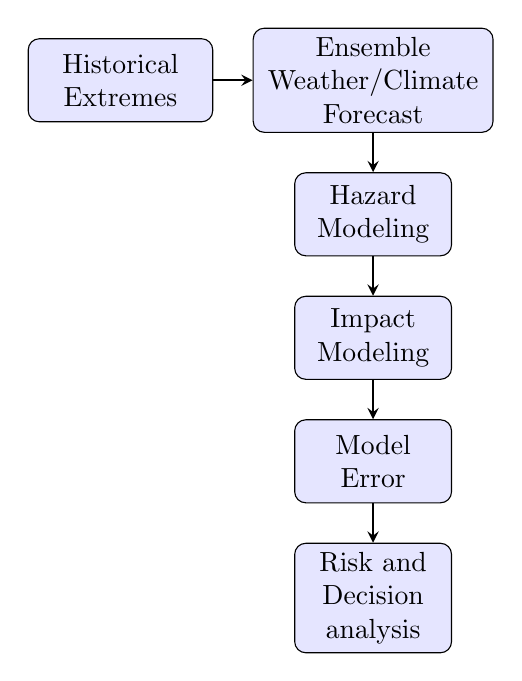
\begin{tikzpicture}
	% Define styles
	\tikzstyle{block} = [rectangle, draw, fill=blue!10, 
	text centered, rounded corners, minimum height=3em]
	\tikzstyle{forecastblock} = [block, text width=8em] % Increased width
	\tikzstyle{otherblock} = [block, text width=5em] % Original width
	\tikzstyle{arrow} = [thick,->,>=stealth]
	
	% Global settings
	\tikzstyle{every node}=[node distance=0.5cm]
	
	% Place nodes
	\node [forecastblock] (forecast) {Ensemble Weather/Climate Forecast};
	\node [block, left=of forecast, text width=6em] (historical) {Historical Extremes}; % New block
	\node [otherblock, below=of forecast] (hazard) {Hazard Modeling};
	\node [otherblock, below=of hazard] (impact) {Impact Modeling};
	\node [otherblock, below=of impact] (error) {Model Error};
	\node [otherblock, below=of error] (risk) {Risk and Decision analysis};
	
	% Draw arrows
	\draw [arrow] (historical) -- (forecast); % New arrow
	\draw [arrow] (forecast) -- (hazard);
	\draw [arrow] (hazard) -- (impact);
	\draw [arrow] (impact) -- (error);
	\draw [arrow] (error) -- (risk);
\end{tikzpicture}
	
\end{frame}

\section{The Role of AI}

\begin{frame}
		\frametitle{The Role of AI in IBF}
	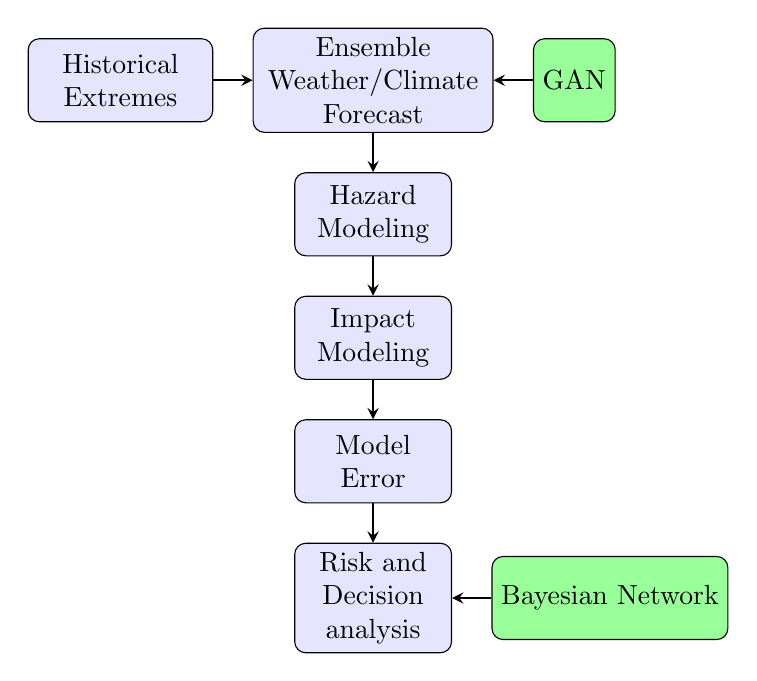
\begin{tikzpicture}
		% Define styles
		\tikzstyle{block} = [rectangle, draw, fill=blue!10, 
		text centered, rounded corners, minimum height=3em]
		\tikzstyle{greenblock} = [rectangle, draw, fill=green!40, 
		text centered, rounded corners, minimum height=3em] % Green block style
		\tikzstyle{forecastblock} = [block, text width=8em] % Increased width
		\tikzstyle{otherblock} = [block, text width=5em] % Original width
		\tikzstyle{arrow} = [thick,->,>=stealth]
		
		% Global settings
		\tikzstyle{every node}=[node distance=0.5cm]
		
		% Place nodes
		\node [forecastblock] (forecast) {Ensemble Weather/Climate Forecast};
		\node [greenblock, right=of forecast] (gan) {GAN}; % GAN block
		\node [block, left=of forecast, text width=6em] (historical) {Historical Extremes}; 
		\node [otherblock, below=of forecast] (hazard) {Hazard Modeling};
		\node [otherblock, below=of hazard] (impact) {Impact Modeling};
		\node [otherblock, below=of impact] (error) {Model Error};
		\node [otherblock, below=of error] (risk) {Risk and Decision analysis};
		\node [greenblock, right=of risk] (bayesian) {Bayesian Network}; % Bayesian Network block
		
		% Draw arrows
		\draw [arrow] (historical) -- (forecast); 
		\draw [arrow] (gan) -- (forecast); % Added arrow from GAN to forecast
		\draw [arrow] (forecast) -- (hazard);
		\draw [arrow] (hazard) -- (impact);
		\draw [arrow] (impact) -- (error);
		\draw [arrow] (bayesian) -- (risk); % Added arrow from GAN to forecast
		\draw [arrow] (error) -- (risk);
	\end{tikzpicture}
\end{frame}


\begin{frame}
	\frametitle{The Role of AI: Post Processing of Ensemble weather forecast}
	
	Generative AI, Generative Adversarial Network (GAN) for Ensemble weather forecasting post process.
	
    \textcolor{blue}{\textbf{Opportunities}}
    \begin{itemize}
    	\item Better bias correction and computationally improved down scaling
    	\item Promising preliminary results 
    	 
    \end{itemize}
    
    \textcolor{blue}{\textbf{Challenges}}
    \begin{itemize}
    	 \item Observation data availability
    	\item Challenges in processing large data sets and routine operation 
    \end{itemize}
   
\end{frame}


\begin{frame}
	\frametitle{GAN model for East Africa Region}
	%	\begin{figure}
		%		\includegraphics[width=1.0\linewidth]{ensemble_weather_forecast.png} 
		%		%\caption{Typical output of IBF}
		%	\end{figure}
	
	\begin{tikzpicture}[remember picture,overlay]
		\node[anchor=north west, inner sep=22pt] at (current page.north west) {
			\includegraphics[width=0.65\linewidth]{gan_ai1.png}
		};
	\end{tikzpicture}
	
\end{frame}


\begin{frame}
	\frametitle{The Role of AI: Bayesian Network for Risk and Decision Analysis}
	
%	The Bayesian Network (BN), representing the interrelations of a set of variables
%	graphically, offers a systematic approach to probabilistic reasoning about uncertainty.
%	This study explores its implementation within IBF
%	
%	\textcolor{blue}{\textbf{Opportunities}}
%	
%	\textcolor{blue}{\textbf{Challenges}}
The Bayesian Network (BN), graphical representation of the interrelations of set of variables , offers a systematic approach to probabilistic reasoning about uncertainty*.
%	This study explores its implementation within IBF

\textcolor{blue}{\textbf{Opportunities}}
\begin{itemize}
	\item ChatGPT application makes BN creation and modeling easy, simple natural language access to model
	\item A tool to record the decision and improve it iteratively  
	
\end{itemize}


\textcolor{blue}{\textbf{Challenges}}
\begin{itemize}
	\item One layer of new method for co production 
\end{itemize}
\end{frame}

\begin{frame}
	\frametitle{BN workflow}
	%	\begin{figure}
		%		\includegraphics[width=1.0\linewidth]{ensemble_weather_forecast.png} 
		%		%\caption{Typical output of IBF}
		%	\end{figure}
	
	\begin{tikzpicture}[remember picture,overlay]
		\node[anchor=north west, inner sep=18pt] at (current page.north west) {
			\includegraphics[width=1.1\linewidth]{BN-model-IBF-v3.png}
		};
	\end{tikzpicture}

\vspace{10em}
\footnotesize{Poster Presentation on 25th Oct 2023 (Wednesday), How do Bayesian Networks support impact-based forecasting for informed decision-making?\\  PC28, AI for weather and climate extremes}

\end{frame}








\begin{frame}
	\frametitle{Key Takeaways}
	

	\begin{itemize}
		\item Multiple generation of IBF
		\item Role of uncertainty and transparency for Risk mitigation/ Anticipatory action 
		\item Role of AI, GAN and Bayesian Networks 
		
	\end{itemize}
	
	
	
\end{frame}

\begin{frame}{}
	\centering
	Thank you!\\
\end{frame}

%\begin{figure}
%\begin{tikzpicture}[scale=0.9]  % Adjusted the scale for better spacing
%	
%	% Matrix
%	\draw (0,0) grid (4,4);
%	\draw[thick] (4,0) -- (4,4);
%	\draw[thick] (0,0) -- (0,4);
%	
%	% Color fill
%	\fill[green] (0,3) rectangle (1,4);
%	\fill[yellow] (1,3) rectangle (2,4);
%	\fill[brown] (2,3) rectangle (3,4);
%	\fill[red] (3,3) rectangle (4,4);
%	\fill[green] (0,2) rectangle (1,3);
%	\fill[yellow] (1,2) rectangle (2,3);
%	\fill[brown] (2,2) rectangle (3,3);
%	\fill[green] (0,1) rectangle (1,2);
%	
%	% Text
%	\node[font=\small] at (0.5,3.5) {Very low};
%	\node[font=\small] at (1.5,3.5) {Low};
%	\node[font=\small] at (2.5,3.5) {Medium};
%	\node[font=\small] at (3.5,3.5) {High};
%	
%	\node[text width=2cm, align=center, font=\small] at (-0.5,3.5) {High};
%	\node[text width=2cm, align=center, font=\small] at (-0.5,2.5) {Medium};
%	\node[text width=2cm, align=center, font=\small] at (-0.5,1.5) {Low};
%	\node[text width=2cm, align=center, font=\small] at (-0.5,0.5) {Very low};
%	
%	\node[text width=2cm, align=center, font=\small] at (2,-0.5) {Impact};
%	\node[text width=2cm, align=center, rotate=90, font=\small] at (-1.5,2) {Probability};
%	
%	% Legend
%	\draw (5,0) rectangle (6,4);
%	\fill[red] (5,3) rectangle (6,4);
%	\fill[brown] (5,2) rectangle (6,3);
%	\fill[yellow] (5,1) rectangle (6,2);
%	\fill[green] (5,0) rectangle (6,1);
%	
%	\node[align=left, text width=3cm, font=\small] at (7.8,3.5) {Take action};
%	\node[align=left, text width=3cm, font=\small] at (7.5,2.5) {Be prepared};
%	\node[align=left, text width=3cm, font=\small] at (7.5,1.5) {Be aware};
%	\node[align=left, text width=3cm, font=\small] at (7.5,0.5) {No severe Impact};
%	
%\end{tikzpicture}
%\end{figure}



%




%\begin{frame}
%	\frametitle{Title}
%	
%	\begin{columns}
%		
%		% Left column
%		\begin{column}{0.5\textwidth}
%			\begin{itemize}
%				\item Contest 1
%				\item Contest 1
%				\item Contest 1
%				\item Contest 1
%				\item Contest 1
%				\item Contest 1
%			\end{itemize}
%		\end{column}
%		
%		% Right column
%		\begin{column}{0.5\textwidth}
%			\includegraphics[width=0.8\linewidth]{test1.png} \\
%			\tiny \url{https://www.youtube.com/watch?v=RkieV47KPX4} \\
%			\vspace{1cm}
%			\includegraphics[width=0.8\linewidth]{test1.png} \\
%			\tiny \url{https://www.youtube.com/watch?v=RkieV47KPX4}
%		\end{column}
%		
%	\end{columns}
%\end{frame}



\end{document}
